%%%% Weekly Report Information %%%%
\newcommand{\handoutName}{Weekly report}
%\newcommand{\handoutdate}{August 25, 2015}  %use this to hard code the date
\newcommand{\handoutdate}{\today}
\newcommand{\duedate}{}



% Header template used for Weekly Reports
\documentclass[11pt,twoside]{article}

\setlength{\oddsidemargin}{0pt}
\setlength{\evensidemargin}{0pt}
\setlength{\textwidth}{6.5in}
\setlength{\topmargin}{0in}
\setlength{\textheight}{8.5in}
\setlength{\voffset}{0in}

\providecommand{\titlesize}{small}


\usepackage{graphicx}
\usepackage{subfigure}
\usepackage{palatino}
%\usepackage{cmbright}
\newcommand{\myMargin}{1.00in}
%\usepackage[pdftex]{hyperref}
\usepackage[small,bf]{caption}
\usepackage{amsmath}
\usepackage[usenames,dvipsnames]{color}
\usepackage{fancyhdr}
\pagestyle{fancy}
\usepackage{datetime}
\usepackage{fancyvrb}
\usepackage{color}
\usepackage[\titlesize, compact]{titlesec}
\usepackage{multicol}
\usepackage{enumitem}
\usepackage{pdfpages}
\usepackage{mdwlist}

\usepackage[colorlinks=true, urlcolor=blue, pdfborder={0 0 0}]{hyperref}

\newdateformat{dashdate}{\THEYEAR-\twodigit{\THEMONTH}-\twodigit{\THEDAY}}
\def\Tiny{\fontsize{3pt}{3pt}\selectfont}

\providecommand{\handoutName}{Handout title}
\providecommand{\handoutdate}{Handout date}
\providecommand{\duedate}{}

\lhead{Robotic Swarm Control Lab}
\chead{}
\rhead{ $<$LI HUANG$>$\\
\handoutdate }
\lfoot{}
\cfoot{\thepage}
\rfoot{\dashdate \Tiny \textcolor{Gray}{\today}}
\renewcommand{\headrulewidth}{0.4pt}
\renewcommand{\footrulewidth}{0.4pt}

\begin{document}

\vspace{0.60in}
\begin{center}
{\Large\textbf{\handoutName}}\\
\vspace{0.03in}
\textbf{\duedate}\\
\end{center}

\newcommand{\todo}[1]{
  \textcolor{Red}{
    \begin{tabular}{|c|}
      \hline
      \em \large \bfseries todo: \normalfont \normalsize #1 \\
      \hline
    \end{tabular}}
}

%%%%%%%%%%%%%%%%%%%%%%%%%%%%%%%%
\iffalse
{\scriptsize
Weekly reports are to be emailed to atbecker@uh.edu by 5:00pm on Tuesdays.  The purpose of a weekly report is to:
(1) give you text and images for your papers, thesis, and dissertation, (2) document progress, (3) identify if you are stuck or need resources.
}
\fi
%%%%%%%%%%%%%%%%%%%%%%%%%%%%%%%%
\section{My \emph{Goals} from last week}
\begin{itemize}
\item Starting a review of our work on MRI robotics and adding contents to the current version

%%%%%%%%%%%%%%%%%%%%%%%%%%%%%%%%
\iffalse
\item $\ldots$
\fi
\end{itemize}
%%%%%%%%%%%%%%%%%%%%%%%%%%%%%%%%

\section{My \emph{Accomplishments} this week}

\subsection{Project 1: \emph{MRI-powered Robots}}

\begin{itemize}
\item Copied and saved all Latex code corresponding to "MRI-powered Robots" to Github

\iffalse
Deliverables can be documents, code, videos, plots, experiments, etc.	Save and backup all work [code, data, LaTeX, images, videos].  Papers and code should be saved to our git server: \href{github.com/aabecker}{https://github.com/aabecker}.
\fi

\item I highlighted and added $<$3$>$ cases of $<$MRI-powered robots studies$>$ to the review, including commutation control of an actuator, simultaneously powering of many actuators and Gauss gun design and construction. It's going to be my first publication and I'm excited!
\item A couple of images are added here to show parts of my work.

\end{itemize}

\begin{figure}[h]
\begin{center}
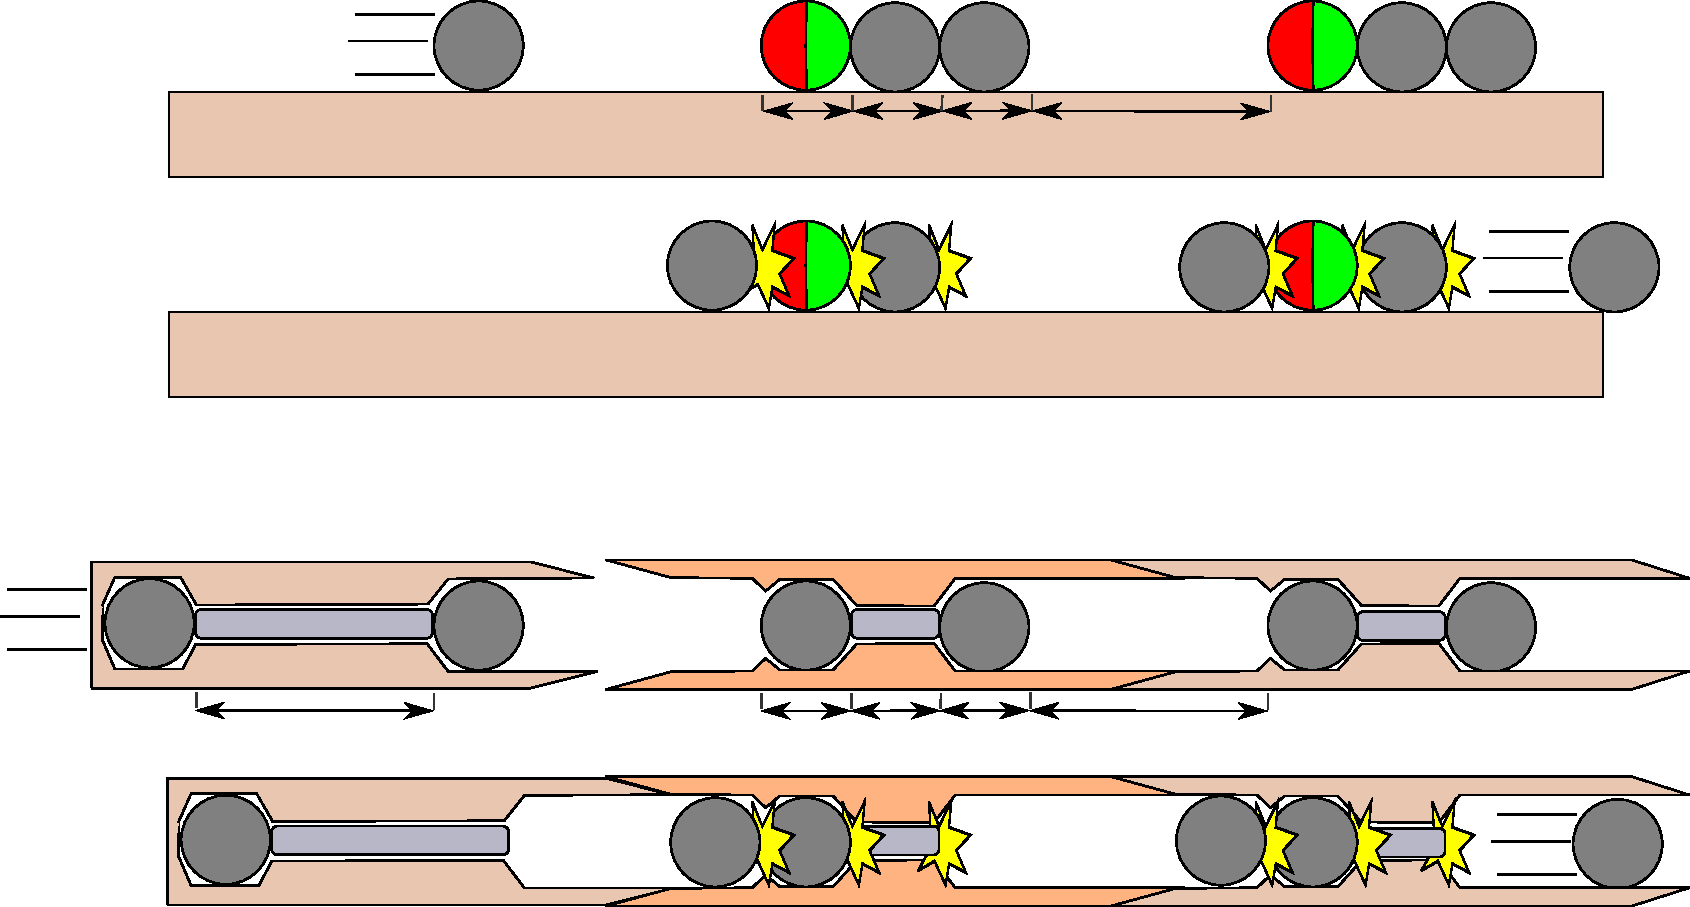
\includegraphics[width=8cm]{fig/GaussGunToyAndMRI}
\caption{Self-assembled Gauss gun}
\end{center}
\end{figure}

\begin{figure}[h]
	\begin{center}
		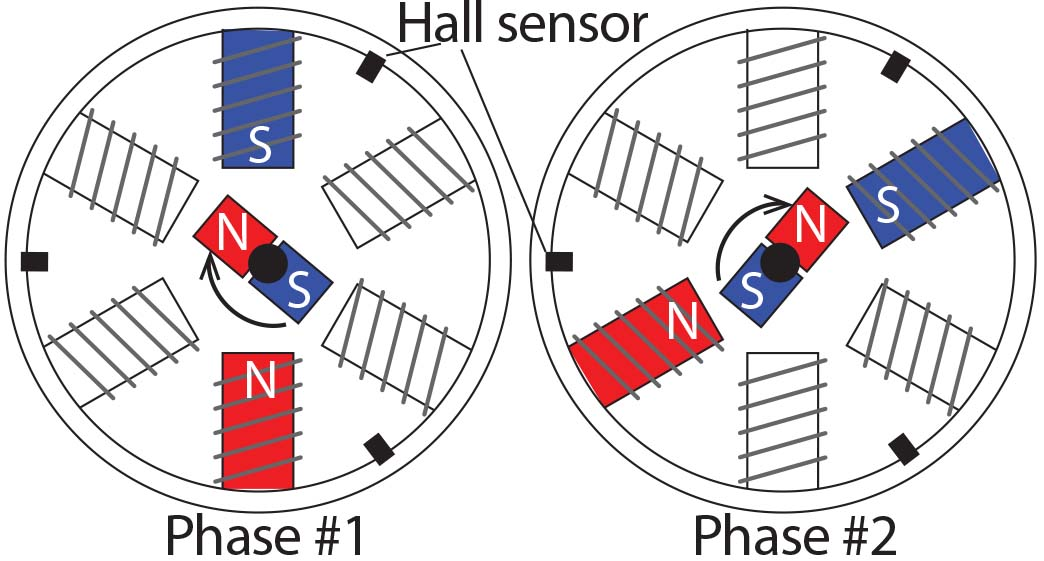
\includegraphics[width=4cm]{fig/CommutationControl1}
		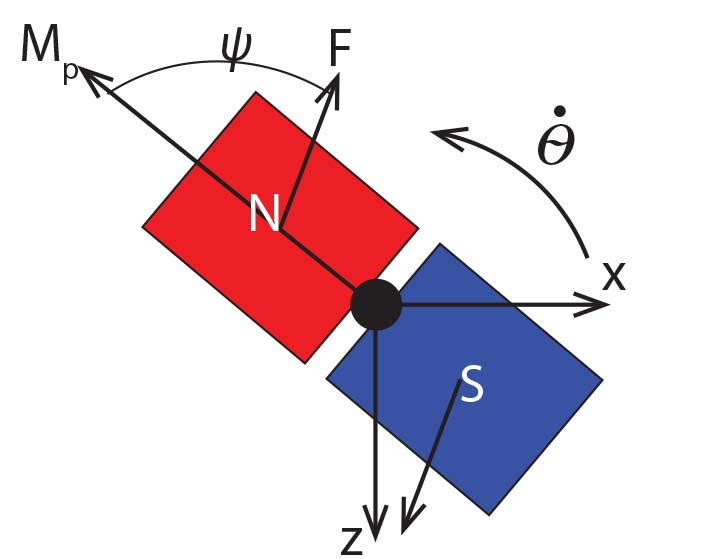
\includegraphics[width=4cm]{fig/CommutationControl2}
		\caption{Commutation Control of an actuator}
	\end{center}
\end{figure}
\subsection{Project 2: \emph{STONES-THROW}}
\begin{itemize}
	\item Set up my robotics research repository and picked up a fancy name.
\end{itemize}


\section{My \emph{Goals} for next week}

\begin{itemize}
\item Finishing theory part and concluding the study on MRI Gauss gun within one page
\end{itemize}

\iffalse

\section{Meeting with Dr. Becker on $<$INSERT DATE and TIME$>$}

What I need Dr. Becker to do:
\begin{itemize}
\item something for Dr. Becker to do
\item $\ldots$
\end{itemize}

\fi

\iffalse

{\tiny
Template available at \href{https://github.com/aabecker/RoboticSwarmControlLab/blob/master/WeeklyReportTemplate/weekly_Report_Template.pdf}{https://github.com/aabecker/RoboticSwarmControlLab/blob/master/WeeklyReportTemplate/weekly\_Report\_Template.pdf}
}
\fi

\end{document}

